\chapter{СУДАЛГААНЫ АРГА ЗҮЙ}

\section{Системийн ерөнхий тойм}

Энэхүү бүлэгт системийн бүтэц, өгөгдлийн урсгал болон pipeline-ийн ажиллагааг 
тайлбарлана. Өгөгдөл цуглуулахаас эхлэн 3D загвар гаргах хүртэлх бүх алхмуудыг 
дарааллан авч үзнэ.

\subsection{Системийн Flow Diagram}

Системийн ажиллагааны үндсэн урсгалыг доорх диаграммаар харуулав:

\begin{figure}[H]
\centering
\begin{tikzpicture}[
    scale=0.95, transform shape,
    node distance=1cm,
    startstop/.style={rectangle, rounded corners, minimum width=2.5cm, minimum height=0.7cm, draw=black, fill=red!20, align=center, font=\small},
    process/.style={rectangle, minimum width=2.5cm, minimum height=0.7cm, draw=black, fill=blue!20, align=center, font=\small},
    decision/.style={diamond, minimum width=2cm, minimum height=0.9cm, draw=black, fill=yellow!20, align=center, aspect=2, font=\small},
    io/.style={trapezium, trapezium left angle=70, trapezium right angle=110, minimum width=2.2cm, minimum height=0.6cm, draw=black, fill=green!20, align=center, font=\small},
    arrow/.style={thick,->,>=stealth}
]
    % Nodes
    \node (start) [startstop] {Эхлэх};
    \node (capture) [io, below=of start] {Олон 2D зураг\\камераар авах};
    \node (preprocess) [process, below=of capture] {Өгөгдлийг цэвэрлэх\\(жишээ: өнгө засах, шилжилт тохируулах)};
    \node (colmap) [process, below=of preprocess] {COLMAP ашиглан\\Feature extraction and Sparse/ Dense reconstruction};
    \node (convert) [process, below=of colmap] {COLMAP файлыг\\OpenMVS форматаар хөрвүүлэх};
    \node (openmvs) [process, below=of convert] {OpenMVS-д ажиллуулах\\Dense reconstruction, Mesh generation, Texture mapping};
    \node (output) [io, below=of openmvs] {3D загварыг .ply, .obj гэх мэт форматаар гаргах};
    \node (end) [startstop, below=of output] {Дуусах};

    % Arrows
    \draw [arrow] (start) -- (capture);
    \draw [arrow] (capture) -- (preprocess);
    \draw [arrow] (preprocess) -- (colmap);
    \draw [arrow] (colmap) -- (convert);
    \draw [arrow] (convert) -- (openmvs);
    \draw [arrow] (openmvs) -- (output);
    \draw [arrow] (output) -- (end);
\end{tikzpicture}
\caption{Ажиллагааны Flow Diagram}
\label{fig:flow_diagram}
\end{figure}

\clearpage
\subsection{Өгөгдөл цуглуулах арга}

Туршилтад нийтэд нээлттэй датасетүүд болон видео бичлэг ашигласан. 1-р туршилтад Temple Ring датасетийн 47 зургийг ашигласан ($360°/47\approx 7.7°$-ийн алхамтай, $1920\times1080$, JPEG). 2-р туршилтад Caterpillar датасет (${\sim}380$ зураг) ашигласан. 3-р туршилтад нийтэд нээлттэй Lighthouse 4K бичлэгээс (5:45 урт, 23.98\,fps, $4096\times2160$) 4с, 2с, 1.5с давтамжаар ${\sim}86$, ${\sim}172$, ${\sim}200$ фрейм гаргаж авсан. Эдгээр датасетийг зохиогч бүтээгээгүй болно.

\textbf{Датасетийн задаргаа:} Туршилт тус бүрт ашигласан датасетийн задаргааг доорх хүснэгтэд харуулав.

\begin{table}[H]
\centering
\caption{Туршилтын датасетийн тойм}
\label{tab:dataset_summary}
\begin{tabular}{|l|c|l|}
\hline
\textbf{Датасет} & \textbf{Зургийн тоо} & \textbf{Ашиглагдсан туршилт} \\ \hline
Temple Ring & 47 & 1-р туршилт \\ \hline
Caterpillar & ${\sim}380$ & 2-р туршилт \\ \hline
Lighthouse 4K видео & ${\sim}86$ / ${\sim}172$ / ${\sim}200$ фрейм & 3-р туршилт \\ \hline
\end{tabular}
\end{table}

\subsection{Урьдчилсан боловсруулалт}
Зургуудыг SfM болон MVS алгоритмуудын шаардлага хангахаар урьдчилан боловсруулав. Үүнд:
\begin{itemize}
    \item Зургийн хэмжээг нэг стандартад тааруулж дахин хэмжээсжүүлсэн;
    \item Хэрэв шаардлагатай бол Gaussian blur removal болон дэнситэйжүүлэлт хийсэн;
    \item Өнгөний тогтвортой байдлыг хангах зорилгоор white balance болон color normalization хийсэн;
    \item Датасетийн зургууд нэг нарийвчлал, ижил форматтай тул өнгөний тогтвортой байдал хангалттай байсан.
\end{itemize}
Эдгээр алхмууд нь фичер илрүүлэлт болон тохиролтын чанарыг шууд сайжруулах зорилготой.

\subsection{Фичер илрүүлэлт ба тохиролт (SIFT)}
Энэхүү ажилд COLMAP-ийн \texttt{feature\_extractor} командаар SIFT алгоритмыг 
ашиглан keypoint илрүүлж, descriptor үүсгэсэн. Камерын загварыг PINHOLE гэж 
тохируулсан нь дотоод параметрийг зөв боловсруулахад тусалсан.
Фичер тохиролтыг COLMAP-ийн \texttt{exhaustive\_matcher} ашиглан хийсэн бөгөөд энэ 
арга нь зургийн бүх боломжит хослолыг хооронд нь тулгаж, хамгийн найдвартай 
тохиролтуудыг сонгодог. Гэсэн хэдий ч зарим нөхцөлд хязгаарлалт ажиглагдсан.
Тухайлбал, зургуудын харагдах талбай хязгаарлагдмал буюу хоорондын өнцгийн
ялгаа их байх үед зарим хослолын хооронд найдвартай тохиролт олж чадахгүй байсан.
Энэ нь sparse reconstruction-ийн бүрэн бүтэн байдалд нөлөөлж, цэгэн үүлний
нягтралыг бууруулах эрсдэлтэй. Цаашдын судалгаанд SuperPoint зэрэг нейрон 
сүлжээний суурьтай фичер илрүүлэгчийг ашиглах нь энэ асуудлыг шийдвэрлэх 
боломжтой гэж үзэж байна.

\subsection{Камерын параметр тооцоолол}
Энэхүү ажилд камерын intrinsic параметрүүдийг COLMAP-ийн дотоод auto-calibration механизмаар тооцоолсон — тухайлбал, PINHOLE загварын хувьд фокусын урт болон гол цэгийг (principal point) SfM-ийн bundle adjustment-ын явцад автоматаар тодорхойлдог. Ашигласан датасетүүд нь нийтэд нээлттэй тул тусдаа checkerboard калибрацийн алхам хийгдээгүй. Extrinsic параметр буюу камер бүрийн байрлал ба чиглэлийг SfM алгоритм тохиролцсон фичерүүд дээр тулгуурлан автоматаар тооцоолно.

Камерын дотоод параметрийн матриц $\mathbf{K}$-г дараах хэлбэрээр бичнэ:

\begin{equation}
\mathbf{K} = \begin{bmatrix} f_x & 0 & c_x \\ 0 & f_y & c_y \\ 0 & 0 & 1 \end{bmatrix}
\label{eq:intrinsic}
\end{equation}

энд $f_x$, $f_y$ нь пикселэр илэрхийлсэн хэвтээ болон босоо тэнхлэгийн фокусын урт, $c_x$, $c_y$ нь зургийн хавтгай дахь оптик тэнхлэгийн проекцийн байрлал буюу голлох цэг (principal point) юм.

Энэхүү ажилд COLMAP-д PINHOLE камерын загварыг сонгосон нь RADIAL эсвэл OPENCV загварыг бус энгийн загварыг ашигласан явдал юм. Тогтмол фокустай, benchmark датасетийн зургуудад линзний гажуудлын нөлөө өчүүхэн байдаг тул PINHOLE загвар хангалттай нарийвчлалтай. Шаардлагагүй нарийн загвар ашиглах нь калибрацийн параметрүүдийг шуугиан дээр хэт тохируулах (overfitting) эрсдэлтэй бөгөөд хуурамч гажуудлын засваруудыг нэмж, реконструкцийн нарийвчлалыг бууруулж болзошгүй юм.

\subsection{Structure-from-Motion (SfM)}
SfM үе шат нь олон зурагнаас камерын байрлал болон sparse point cloud үүсгэнэ. Энэ үе шат дараах алхмуудтай:
\begin{itemize}
    \item Зураг хоорондын best pair сонгох;
    \item Bundle adjustment ашиглан камерын байрлал болон цэгүүдийг нэгэн зэрэг оновчлох;
    \item Essential болон Fundamental matrix тооцоолох;
    \item Камерын эхний байрлал тогтоох;
    \item Инкрементал байдлаар дараагийн зургуудыг нэмэх;
    \item Sparse point cloud үүсгэх.
\end{itemize}
Энэ алхмын гол үр дүн нь объектын үндсэн геометрийн дүрслэл бүхий сийрэг цэгэн загвар юм.

\subsection{Multi-View Stereo (MVS)}
SfM-ээс гарсан камерын байрлал болон сийрэг цэгүүд дээр тулгуурлан нягт (dense) цэгэн өгөгдлийг MVS ашиглан сэргээв. Энэ үе шат нь:
\begin{itemize}
    \item Зураг бүрт depth map тооцоолох;
    \item Зураг хоорондын depth map-уудыг нэгтгэх;
    \item Нягт цэгэн облак үүсгэх.
\end{itemize}
Үр дүнд нь өндөр нарийвчлалтай гадаргуугийн геометр сэргээгдэнэ.

\subsection{Point Cloud цэвэрлэгээ ба шүүлт}
Нягт point cloud нь дуу чимээтэй байдаг тул дараах боловсруулалтуудыг хийсэн:
\begin{itemize}
    \item Statistical Outlier Removal (SOR);
    \item Radius-based filtering;
    \item Normal estimation.
\end{itemize}
Эдгээр цэвэрлэгээ нь mesh reconstruction-ийн чанарт шууд нөлөөлнө.

\subsection{Mesh Reconstruction}
Цэвэрлэгдсэн цэгэн өгөгдлөөс 3D mesh үүсгэхдээ Poisson Surface Reconstruction алгоритм ашигласан. Үүссэн mesh дээр:
\begin{itemize}
    \item Mesh decimation;
    \item Hole filling;
    \item Texture baking
\end{itemize}
хийж, 3D загварын харагдах байдал болон гүйцэтгэлийг сайжруулсан.

\subsection{Гүйцэтгэл ба үнэлгээний арга}

Сэргээгдсэн 3D загварын чанарыг дараах аргуудаар үнэлсэн.

\textbf{Chamfer Distance:} Сэргээгдсэн цэгэн үүл $P$ болон эталон (ground truth) цэгэн үүл $Q$ өгөгдсөн тохиолдолд Chamfer Distance-ийг хоёр чиглэлийн хамгийн ойр хөршийн зайны дундджаар тооцно:

\begin{equation}
\mathrm{CD}(P,\,Q) = \frac{1}{|P|}\sum_{p \in P}\min_{q \in Q}\|p - q\|^2 + \frac{1}{|Q|}\sum_{q \in Q}\min_{p \in P}\|p - q\|^2
\label{eq:chamfer}
\end{equation}

Энэхүү судалгаанд гадаад 3D сканнер байхгүй байсан тул эталон цэгэн үүл $Q$ болгон SIFT + Exhaustive matching тохиргоо (1A) ашиглан үүсгэсэн нягт цэгэн үүлийг ашигласан. Энэ тохиргоо нь 1-р туршилтад хамгийн бага RMSE үзүүлэн хамгийн найдвартай гаралтыг өгсөн тул эталон болгон сонгосон. Туршиж байгаа тохиргоо бүрийн нягт цэгэн үүл нь сэргээгдсэн цэгэн үүл $P$ болно.

\textbf{RMSE (Root Mean Square Error):} RMSE нь харгалзах цэгүүдийн хоорондох дундаж квадрат зайны квадрат язгуурыг хэмждэг. Chamfer Distance нь хоёр чиглэлд хамгийн ойр хөршийг ашигладгаас ялгаатай нь энэхүү судалгааны RMSE нь сэргээгдсэн цэгэн үүлнээс эталон руу чиглэсэн нэг чиглэлийн хамгийн ойр хөршийн зайг тооцоолсны дараа квадрат язгуур авдаг. Утга бага байх тусам сэргээгдсэн загвар геометрийн хувьд эталонтой илүү ойр байна.

\textbf{Харааны үнэлгээ:} Метрик үнэлгээнээс гадна mesh бүрийг цоорхой, гадаргуугийн тасалдал болон геометрийн гажуудлын хувьд харааны аргаар шалгасан. Зарим алдаа нь тоон хэмжүүрт тусгагдахгүй байж болох тул харааны шалгалт нь үнэлгээг нэмэлтээр бүрэн болгодог.

\textbf{COLMAP baseline-тэй харьцуулалт:} Тохиргоо 1A (SIFT + Exhaustive) нь бусад бүх тохиргоог харьцуулах суурь (baseline) болгон ашигласан. Бусад matcher болон хослолын аргуудын үр дүнг энэ baseline-тэй харьцуулан давуу болон сул талуудыг тодорхойлсон.

\subsection{Туршилтын орчин}
Туршилтуудыг дараах техник хангамжийн орчинд гүйцэтгэсэн:
\begin{itemize}
    \item GPU: NVIDIA RTX 4060
    \item CPU: Intel Core i9 (15th Gen)
    \item RAM: 16 GB
    \item Програмын сангууд: COLMAP, OpenMVS, OpenCV, Python, PyQt5, PyYAML
\end{itemize}
Эдгээр үзүүлэлт нь pipeline-ийн хурд, гүйцэтгэлд нөлөөлсөн тул тэмдэглэн авсан.

\clearpage

\subsection{Програм хангамжийн архитектур}

\textbf{Технологийн сонголтын үндэслэл:} Python програмчлалын хэлийг сонгосон нь хурдан прототип бүтээх боломж, COLMAP болон OpenMVS-тэй командын мөрөөр харилцах subprocess интерфейсийн хялбар байдал, мөн машин сургалтын номын сангуудтай (NumPy, Open3D) нэгтгэх ирээдүйн боломжийг харгалзан үзсэн шийдвэр юм. PyQt5-ийг UI framework болгон сонгосон нь энэ нь боловсорч гүйцсэн (mature) фреймворк бөгөөд signal/slot механизм нь pipeline worker thread болон UI-ийн хооронд аюулгүй харилцааг хангадаг учраас юм. YAML тохиргооны систем нь хүний унших боломжтой, код дахин compile хийхгүйгээр exe замыг өөрчлөх боломж олгодог тул ашигласан. Modular бүтэц нь туршилтын янз бүрийн тохиргоог бие даан солих боломжийг бий болгодог.

Системийн архитектурыг доорх диаграммаар харуулав:

\begin{figure}[H]
\centering
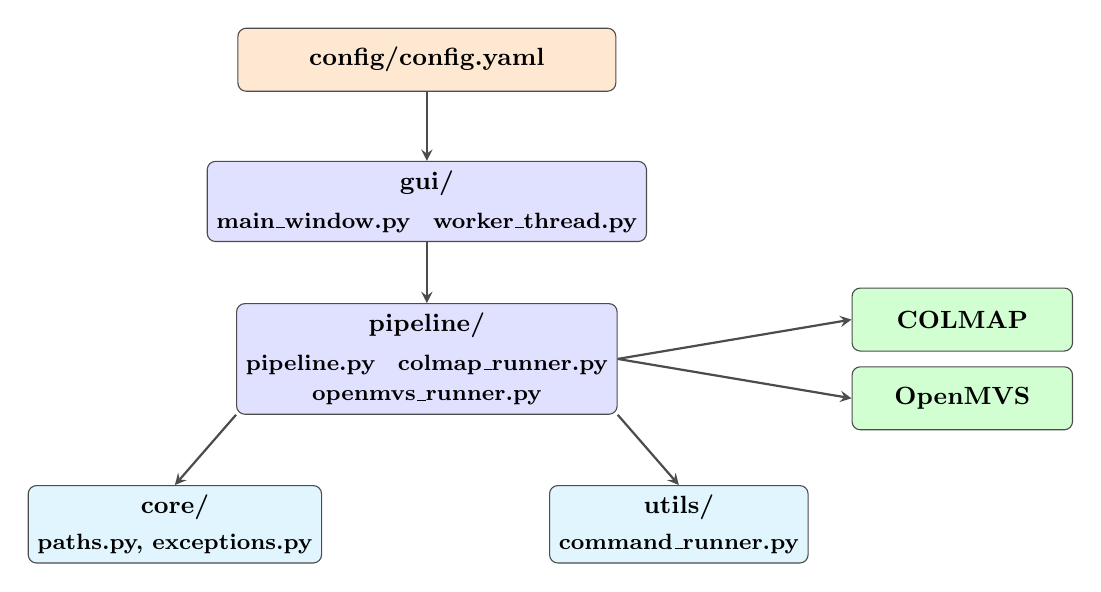
\begin{tikzpicture}[
    appbox/.style={rectangle, rounded corners=3pt, minimum width=4.8cm,
                   draw=black!70, fill=blue!12, align=center, font=\small\bfseries},
    extbox/.style={rectangle, rounded corners=3pt, minimum width=2.8cm, minimum height=0.8cm,
                   draw=black!70, fill=green!18, align=center, font=\small\bfseries},
    cfgbox/.style={rectangle, rounded corners=3pt, minimum width=4.8cm, minimum height=0.8cm,
                   draw=black!70, fill=orange!18, align=center, font=\small\bfseries},
    supbox/.style={rectangle, rounded corners=3pt, minimum width=3.2cm, minimum height=0.8cm,
                   draw=black!70, fill=cyan!12, align=center, font=\small\bfseries},
    arr/.style={->, >=stealth, thick, draw=black!70}
]

%% All nodes placed at explicit absolute coordinates %%

% Vertical stack (x=0)
\node[cfgbox] (cfg)  at (0,  5.3) {config/config.yaml};
\node[appbox] (gui)  at (0,  3.5) {gui/ \\[3pt]
    {\footnotesize main\_window.py \enspace worker\_thread.py}};
\node[appbox] (pip)  at (0,  1.5) {pipeline/ \\[3pt]
    {\footnotesize pipeline.py \enspace colmap\_runner.py} \\
    {\footnotesize openmvs\_runner.py}};

% Support modules — placed below pip, spread left/right
\node[supbox] (core)  at (-3.2, -0.6) {core/ \\[2pt]
    {\footnotesize paths.py, exceptions.py}};
\node[supbox] (utils) at ( 3.2, -0.6) {utils/ \\[2pt]
    {\footnotesize command\_runner.py}};

% External tools — placed to the right of pip
\node[extbox] (colmap) at (6.8,  2.0) {COLMAP};
\node[extbox] (omvs)   at (6.8,  1.0) {OpenMVS};

%% Arrows %%

% Vertical chain: config → gui → pipeline
\draw[arr] (cfg.south)  -- (gui.north);
\draw[arr] (gui.south)  -- (pip.north);

% Pipeline → external tools
\draw[arr] (pip.east)       -- (colmap.west);
\draw[arr] (pip.east) -- (omvs.west);

% Pipeline → support modules
\draw[arr] (pip.south west) -- (core.north);
\draw[arr] (pip.south east) -- (utils.north);

\end{tikzpicture}
\caption{Системийн програм хангамжийн модульд суурилсан архитектурын диаграмм}
\label{fig:software_architecture}
\end{figure}

Дипломын ажлын хэрэгжүүлэлт нь Python програмчлалын хэл дээр бичигдсэн бөгөөд дараах модульд хуваагдан зохион байгуулагдсан:

\begin{itemize}
    \item \textbf{core/} — суурь бүрэлдэхүүнүүд: ажлын замын тодорхойлолт (\texttt{paths.py}), алдааны ангилал (\texttt{exceptions.py}), лог бичилт (\texttt{logger.py})
    \item \textbf{pipeline/} — COLMAP болон OpenMVS-тэй харилцах модулиуд:
    \begin{itemize}
        \item \texttt{pipeline.py} — 9 үе шаттай ерөнхий pipeline удирдлага
        \item \texttt{colmap\_runner.py} — COLMAP командуудыг дуудах wrapper
        \item \texttt{openmvs\_runner.py} — OpenMVS командуудыг дуудах wrapper
        \item \texttt{model\_converter.py} — гаралтын файлуудыг цуглуулах
    \end{itemize}
    \item \textbf{gui/} — хэрэглэгчийн графикийн интерфейс (PyQt5):
    \begin{itemize}
        \item \texttt{main\_window.py} — үндсэн цонх болон удирдлагын элементүүд
        \item \texttt{worker\_thread.py} — pipeline-ийг ар талд ажиллуулах тусдаа thread
        \item \texttt{styles.qss} — интерфейсийн харааны загварчлал
    \end{itemize}
    \item \textbf{utils/} — туслах хэрэгслүүд: гадаад програм ажиллуулагч (\texttt{command\_runner.py})
    \item \textbf{config/config.yaml} — гүйцэтгэлийн файлуудын зам болон тохиргоог YAML форматаар хадгалах
\end{itemize}

PyQt5-д суурилсан GUI нь дараах боломжуудыг хэрэглэгчид олгоно:

\begin{itemize}
    \item Зургийн хавтас болон ажлын хавтасны замыг шалгаж сонгох
    \item GPU ашиглалт, mesh сайжруулалт (Refine Mesh), текстур зураглал (Texture Mesh)-ийг идэвхжүүлэх буюу унтраах
    \item 9 үе шаттай дэвшлийн мөр (progress bar) болон тайлбарт статус харуулагч
    \item Бодит цагийн лог цонх — pipeline-ийн гаралтыг шууд дэлгэцэнд харуулах
    \item Pipeline-ийг зогсоох (Abort) болон ажлын хавтасыг цэвэрлэх (Clean Workspace) товчлуурууд
    \item Амжилттай дууссаны дараа гаралтын хавтасыг нээх товч
\end{itemize}

Worker thread нь pipeline-ийн хүнд тооцооллыг үндсэн GUI thread-ийг хааж болохгүй тул тусдаа thread дээр ажиллуулна. Хэрэглэгч Abort товч дарсан тохиолдолд ажиллаж байгаа COLMAP буюу OpenMVS процессыг аюулгүйгээр зогсоож, хагас боловсруулагдсан файлуудыг устгах боломж олгоно.

Pipeline-ийн тохиргоог \texttt{config/config.yaml} файлаар удирдана. Тус файлд COLMAP болон OpenMVS-ийн гүйцэтгэлийн файлуудын зам, ажлын хавтас болон GPU, refine, texture зэрэг тохиргоонуудыг YAML форматаар хадгалдаг бөгөөд GUI-ийн "Save Config" товчоор шинэчлэнэ.

\clearpage

\begin{figure}[htbp]
\centering
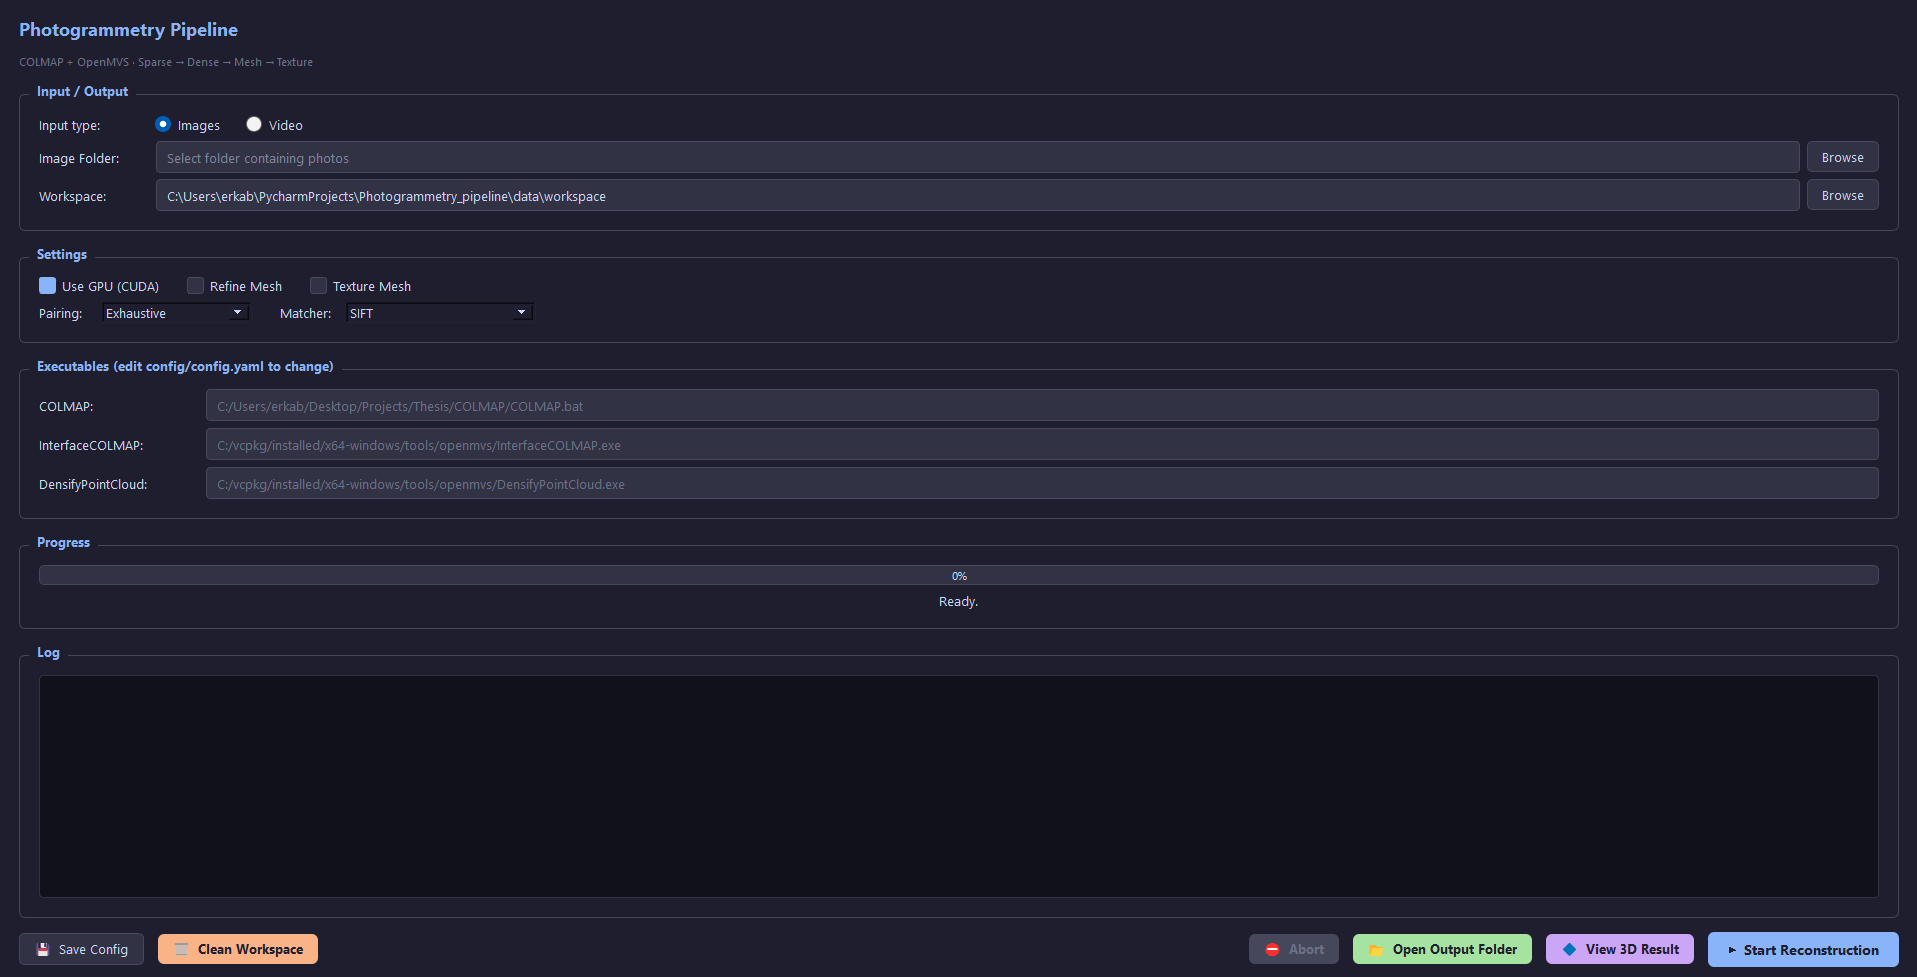
\includegraphics[width=0.9\textwidth]{Pictures/UpdatedGUI.png}
\caption{PyQt5 GUI ашигласан pipeline удирдлага}
\label{fig:GUI_appearance}
\end{figure}

\begin{figure}[htbp]
\centering
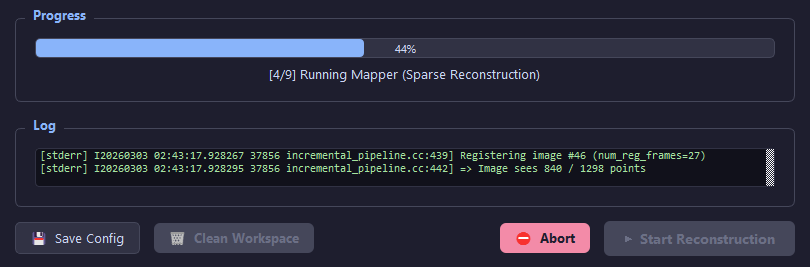
\includegraphics[width=0.9\textwidth]{Pictures/GUI_working.png}
\caption{GUI pipeline ажиллаж байх үеийн дэвшлийн мөр болон лог цонх}
\label{fig:GUI_working}
\end{figure}

\clearpage

